% ================================================================================================ capítulo 2
\chapter{Medición del seeing}\label{cap:medicion}

\begin{resumen}
\textbf{En este capítulo:} las cinco páginas del modo medición (\menu{Video}, \menu{Recorte y tramo},
\menu{Parámetros}, \menu{Procesar} y \menu{Resultados}), cómo guardar y exportar, y el \menu{Historial}. Si mides con
un equipo que no es del OAN, lee también el capítulo~\ref{cap:propio}.
\end{resumen}

El modo medición sigue el orden en que se hace el trabajo: cargar el video, decir dónde está la estrella, dar los
datos del equipo, procesar y leer los resultados. Los pasos están numerados en el menú de la izquierda; puedes saltar
entre ellos cuando quieras y nada se pierde.

% ------------------------------------------------------------------------------------------------ 1. Video
\section{Video}\label{sec:video}

Arrastra el video a la ventana o haz clic en el recuadro para buscarlo. TurbuLENS lee los formatos de las cámaras de
fotos y de los celulares (MOV, MP4, MTS, AVI, MKV, WMV, WebM\ldots), los de las cámaras astronómicas (SER, AVI sin
compresión, cubos FITS) y videos de 16 bits. El video no se copia: se lee desde su carpeta cada vez que hace falta, así
que un archivo de varios gigabytes no ocupa espacio extra.

\begin{capturam}{video}{La página \menu{Video} con un video cargado.}
\item El \textbf{primer cuadro} del video, para confirmar que es el correcto.
\item \textbf{Información del video}: formato, resolución, cuadros por segundo, número de cuadros, duración,
profundidad (8 o 16 bits) y tamaño del archivo.
\item \boton{Cambiar video} abre otro.
\item \botonp{Siguiente: recorte y tramo} pasa al paso 2.
\end{capturam}

\begin{nota}[¿Qué video sirve?]
Uno de 20 a 120 segundos de una estrella brillante (Vega, Altair, Sirio, Canopus, Arturo\ldots) con la máscara del DIMM
puesta y el telescopio un poco desenfocado, de modo que se vean \textbf{dos puntos separados}. Mientras más cuadros por
segundo y menos compresión, mejor. La exposición de cada cuadro debe ser corta (1/250~s o menos si la cámara lo
permite): con exposiciones largas la turbulencia se promedia dentro del cuadro y el seeing sale menor de lo real
(sección~\ref{sec:sesgos}).
\end{nota}

% ------------------------------------------------------------------------------------------------ 2. Recorte
\section{Recorte y tramo}\label{sec:recorte}

Aquí dices \textbf{dónde} está la estrella (la región) y \textbf{qué parte} del video se usa (el tramo). La estrella ocupa
unas decenas de píxeles de una imagen de dos millones: medir solo esa zona hace el análisis cientos de veces más
rápido y los archivos cientos de veces más livianos.

\begin{capturam}{region}{\menu{Recorte y tramo}. La región, en línea discontinua, encierra los dos puntos con margen.}
\item \textbf{El cuadro del video} con la región. Se dibuja y se ajusta como en Paint (tabla~\ref{tab:region}).
\item \boton{◎ Ajustar a la estrella} busca la imagen doble y pone la región a su alrededor. \campo{Tamaño rápido…}
da tamaños fijos (48 a 256~px) o el cuadro completo.
\item \campo{Seguir a la estrella}: la región se recentra en cada cuadro.
\item \campo{Tamaño automático}: el tamaño de la región se ajusta a los puntos al procesar.
\item \textbf{Zoom} de la vista: 1× a 16×.
\item \textbf{Dentro de la región}, ampliado, con un aviso de estado y la posición y el tamaño exactos en píxeles.
\item \textbf{Línea de tiempo} con la entrada y la salida del tramo.
\item \boton{[ Entrada} y \boton{Salida ]} marcan el tramo en el cuadro que estás viendo; \boton{Todo} usa el video
completo; \campo{Ir a} salta a un cuadro (1820) o a un tiempo (01:05.5).
\item \textbf{Reproducción}: \boton{<<} y \boton{>>} reproducen hacia atrás o hacia adelante a velocidad constante
(0,25× a 32× del video real); \boton{<} y \boton{>} avanzan un cuadro.
\end{capturam}

\begin{table}[H]
\centering\small
\begin{tabularx}{\linewidth}{@{}l Y@{}}
\toprule
Acción & Qué hace\\
\midrule
Arrastrar en la imagen & Dibuja una región nueva.\\
Arrastrar desde dentro de la región & La mueve.\\
Arrastrar los cuadritos blancos & Cambia su tamaño.\\
Un clic & Centra la región en ese punto.\\
Rueda del ratón & Acerca o aleja alrededor del cursor.\\
Clic derecho (o central) y arrastrar & Mueve la vista.\\
\tecla{←}\tecla{→}\tecla{↑}\tecla{↓} & Mueven la región un píxel.\\
\tecla{Mayús}\,+\,flechas & Agrandan o achican la región un píxel por lado.\\
\tecla{←}\,\tecla{→} sobre la línea de tiempo & Un cuadro atrás o adelante; con \tecla{Mayús}, un segundo.\\
\bottomrule
\end{tabularx}
\caption{Cómo se maneja la región y la línea de tiempo.}\label{tab:region}
\end{table}

\subsection{El aviso de la región}

Debajo de la vista ampliada, un aviso de color dice si la región sirve. TurbuLENS busca los dos puntos en el cuadro que
estás viendo y comprueba el margen:

\begin{center}\small
\begin{tabularx}{\linewidth}{@{}>{\color{acento}\bfseries}l Y@{}}
Contiene los dos puntos ✓ & Lista para procesar.\\
\textcolor{cobre}{Muy ajustada} & Los puntos caben, pero con menos de 8~px de margen: la turbulencia puede sacarlos.\\
\textcolor{cobre}{Región muy grande} & Funciona, pero los cuadros guardados pesan de más. Pulsa \boton{◎ Ajustar a la estrella}.\\
\textcolor{cobre}{Región muy pequeña} & Con \campo{Tamaño automático} se agranda sola al procesar; sin él, agrándala
(mínimo 16~px).\\
\textcolor{red!70!black}{No se ven los dos puntos} & La estrella no está en la región en este cuadro, o se ve un solo punto.\\
\end{tabularx}
\end{center}

\subsection{Seguir a la estrella y tamaño automático}

Un telescopio sin motor de seguimiento deja que la estrella cruce la imagen: en el video de Altair del grupo, la
estrella se desplaza unos 110~px en horizontal y 140~px en vertical en dos minutos. Con \campo{Seguir a la estrella},
antes de medir TurbuLENS ubica la estrella aunque la región haya quedado lejos (si hace falta la busca en todo el
cuadro) y, cuadro a cuadro, mueve la región hacia el centro de la luz. El movimiento está amortiguado a la mitad para no
copiar el temblor de la turbulencia, y si la estrella se pierde cinco cuadros seguidos, se busca otra vez en todo el
cuadro. Mientras reproduces, la región sigue a la estrella en vivo.

Con \campo{Tamaño automático}, TurbuLENS mide en los primeros cuadros la separación de los puntos, su tamaño y cuánto se
mueve la pareja, y ajusta el lado de la región para que quepan con margen. Las dos opciones vienen marcadas y conviene
dejarlas así.

\subsection{Elegir el tramo}

El tramo es la parte del video que se mide. Déjale fuera el principio y el final si moviste el telescopio al grabar,
y cualquier momento con nubes, un golpe o una ráfaga de viento. Arriba a la derecha se lee la duración y el número de
cuadros del tramo, con un aviso si dura menos de 15~segundos. Más cuadros no siempre es mejor: diez segundos limpios
valen más que un minuto con golpes. En la sección~\ref{sec:incertidumbre} se explica cuántos cuadros hacen falta.

% ------------------------------------------------------------------------------------------------ 3. Parámetros
\section{Parámetros}\label{sec:parametros}

Esta página tiene los datos que convierten píxeles en segundos de arco: la máscara ($D$ y $B$), la longitud de onda
($\lambda$) y la \textbf{escala de placa}. Además decide qué imágenes se guardan y si se calibra cada cuadro con un dark y
un flat.

\begin{capturam}{parametros}{\menu{Parámetros} después de elegir el Celestron 8SE, la Nikon D5600 en video y la máscara del
grupo en \boton{Dispositivos}.}
\item \botonp{Dispositivos (OAN y propios)…} llena todo con un clic: telescopio, cámara y máscara.
\item $D$ y $B$: diámetro de cada orificio y separación entre sus centros, con la unidad que prefieras.
\item $\lambda$: longitud de onda efectiva (550~nm para una cámara a color o sin filtro).
\item \boton{Calcular…} abre la calculadora de la escala de placa; el resultado va en el campo de al lado.
\item \campo{Conozco la altura de la estrella}: para el seeing en el cenit.
\item \textbf{Perfil}: guarda o carga un montaje completo.
\item \campo{Guardar los cuadros como imágenes}.
\item Formato de los cuadros: PNG, TIFF de 16 bits, JPG, NumPy o FITS, y cada cuántos cuadros se guarda uno.
\item Carpeta de salida y espacio que van a ocupar.
\item \campo{Restar el dark y dividir por el flat antes de medir}.
\end{capturam}

\subsection{La máscara y la longitud de onda}

Cada campo numérico tiene al lado su selector de unidad (µm, mm, cm o m; TurbuLENS recuerda la que elegiste) y el rango
que acepta, que también aparece al dejar el cursor encima. Los decimales se pueden escribir con punto o con coma.

\begin{table}[H]
\centering\small
\begin{tabular}{@{}l l l@{}}
\toprule
Dato & Rango permitido & Valor típico\\
\midrule
$D$, diámetro de cada orificio & 0,1 a 100~cm & 2,5 a 5~cm\\
$B$, separación entre centros & 0,2 a 300~cm, y mayor que $D$ & 10 a 20~cm\\
$\lambda$, longitud de onda & 300 a 1100~nm & 550~nm (visible); 650~nm con filtro rojo\\
Altura de la estrella & 5° a 90° & la del momento de grabar\\
\bottomrule
\end{tabular}
\caption{Datos de la máscara y de la observación.}
\end{table}

Si ya procesaste, al cambiar $D$, $B$, $\lambda$, la escala o la altura los resultados se recalculan al instante: no hace
falta procesar otra vez. Es útil para ver cuánto cambia el seeing con una escala u otra.

\subsection{La escala de placa}\label{sec:escala_app}

La escala de placa dice cuántos segundos de arco del cielo caben en un píxel del video. \textbf{Es el dato que más pesa en
el resultado}: el seeing es proporcional a la escala elevada a 6/5 (sección~\ref{sec:escala_teoria}), así que un error
del 10\,\% en la escala da un error del 12\,\% en el seeing. Hay tres maneras de obtenerla:
\begin{enumerate}
\item \textbf{Con \boton{Dispositivos}}, si tu equipo está en la lista o lo agregas (capítulo~\ref{cap:propio}).
\item \textbf{Con la calculadora} (\boton{Calcular…}): elige la cámara o escribe el ancho del sensor, marca
\campo{Grabé en video} si es una cámara de fotos o un celular, escribe la focal del telescopio y pulsa \boton{Usar}. La
calculadora muestra la cuenta completa, con el píxel efectivo del video.
\item \textbf{Midiéndola con el cielo}, con una estrella doble o dejando que una estrella cruce la imagen
(sección~\ref{sec:medir_escala}). Es lo más exacto.
\end{enumerate}

\captura[0.92\linewidth]{parametros_calculadora.png}{La calculadora de la escala de placa: con la Nikon D5600 en video,
el píxel efectivo es el ancho del sensor dividido entre el ancho del video.}

\begin{cuidado}[Cámaras de fotos y celulares.]
Al grabar video, una cámara de fotos o un celular reduce la imagen completa del sensor a 1920 (o 1280) píxeles de ancho.
Cada píxel del video abarca entonces varios píxeles del sensor, y la escala hay que calcularla con el \textbf{píxel
efectivo}: ancho del sensor ÷ ancho del video. Con la Nikon D5600 en el 8SE, la escala correcta es 1,242″/px; con el
píxel del sensor saldría 0,398″/px y el seeing, casi cuatro veces menor de lo real. Las cámaras astronómicas (QHY, ZWO)
graban con los píxeles reales y no tienen este problema.
\end{cuidado}

Sin escala de placa \textbf{no se puede procesar}: el seeing no tendría sentido. \menu{Procesar} lo avisa y tiene un
botón que lleva de vuelta a esta página.

\subsection{Perfiles}

Un perfil guarda $D$, $B$, $\lambda$, la escala, el tamaño de píxel y la focal de un montaje con un nombre («8SE + Nikon,
máscara del grupo»). Elegirlo en la lista carga sus valores. \boton{Guardar…} crea uno nuevo con lo que ves en
pantalla, y el botón \boton{⋯} tiene \menu{Actualizar con los valores actuales} (así se edita), \menu{Renombrar…} y
\menu{Eliminar}. Los perfiles son los mismos en el modo medición y en el educativo.

\subsection{Imágenes a guardar}

TurbuLENS puede guardar cada cuadro del tramo recortado a la región (y centrado en la estrella si la sigues):
\begin{itemize}
\item \textbf{PNG} (recomendado): sin pérdida y el más liviano para medir.
\item \textbf{TIFF de 16 bits}: conserva toda la profundidad de las cámaras astronómicas.
\item \textbf{JPG}: el más liviano, pero altera los píxeles; no lo recomendamos para medir.
\item \textbf{NumPy} o \textbf{FITS}: un solo archivo con todos los cuadros (un cubo), listo para Python o para DS9.
\end{itemize}
Con \campo{Guardar 1 de cada $n$ cuadros} se guarda solo una muestra; la medición usa todos los cuadros igual. Debajo
se ve cuántas imágenes se van a guardar, de qué tamaño y cuánto espacio ocupan. En la carpeta de salida quedan además
\ruta{mediciones.csv} (una fila por cuadro) y \ruta{resumen.json} (los parámetros y el resultado).

\subsection{Calibración con dark y flat}

Si tienes un dark, un flat o un bias \textbf{maestros} del mismo tamaño que el video (se crean en el modo Imágenes,
capítulo~\ref{cap:imagenes}), marca \campo{Restar el dark y dividir por el flat antes de medir} y elige los archivos.
Cada cuadro se corrige como $(\text{cuadro} - \text{dark}) / \text{flat}$ antes de buscar los puntos. Si un maestro no
mide lo mismo que el video, el campo lo avisa con «No coincide con el video». Para el seeing la calibración casi nunca
cambia el resultado (el DIMM mide posiciones, no brillos), pero ayuda con cámaras ruidosas o con píxeles calientes cerca
de la estrella.

% ------------------------------------------------------------------------------------------------ 4. Procesar
\section{Procesar}\label{sec:procesar}

\menu{Procesar} resume lo que se va a hacer (video, tramo, cuadros, región, calibración, imágenes, escala y carpeta) y
tiene un solo botón: \botonp{▶ Iniciar}. La barra muestra los cuadros por segundo y el tiempo que falta; \boton{■ Cancelar}
detiene sin perder lo que ya se midió. Al terminar, TurbuLENS pasa solo a \menu{Resultados}.

\captura{procesar.png}{\menu{Procesar}, listo para empezar. A la derecha, el resumen de lo que se va a medir.}

La velocidad depende sobre todo de decodificar el video y del tamaño de la región. Los puntos se buscan en bloques de cuadros a la vez, con NumPy, sin recorrer los
píxeles uno a uno (sección~\ref{sec:codigo_deteccion}).

\captura[0.85\linewidth]{procesar_sin_escala.png}{Sin escala de placa, \menu{Procesar} no deja empezar y explica por qué.}

% ------------------------------------------------------------------------------------------------ 5. Resultados
\section{Resultados}\label{sec:resultados}

\begin{capturam}{resultados}{\menu{Resultados} de un video de prueba de 600 cuadros.}
\item \textbf{Seeing estimado}, con su calidad en palabras y en color.
\item Seeing \textbf{longitudinal} y \textbf{transversal}, calculados por separado.
\item \textbf{Parámetro de Fried} $r_0$.
\item \textbf{Cuadros usados} y cuántos se descartaron.
\item \textbf{Centroides cuadro a cuadro}: la animación de lo que midió TurbuLENS.
\item \textbf{Histograma} de la separación entre los dos puntos.
\item \textbf{Etiqueta} para el historial (opcional).
\item \botonp{Guardar en historial}.
\end{capturam}

\subsection{Los indicadores}

Cada indicador tiene su botón \textbf{!} con la explicación. En resumen:

\begin{table}[H]
\centering\small
\begin{tabularx}{\linewidth}{@{}l Y@{}}
\toprule
Indicador & Qué es y cómo leerlo\\
\midrule
Seeing estimado & El promedio del longitudinal y el transversal, en segundos de arco. Hasta 1,5″
\textcolor{acento}{\textbf{excelente}}, hasta 3″ \textcolor{cobre}{\textbf{aceptable}}, más de 3″
\textcolor{red!70!black}{\textbf{muy turbulento}}.\\
Seeing longitudinal / transversal & El seeing calculado con el movimiento a lo largo de la línea que une los orificios
y con el perpendicular. Deben parecerse; si difieren mucho, hay algo que no es turbulencia (sección~\ref{sec:controles}).\\
Parámetro de Fried $r_0$ & El tamaño de una «celda» de aire en la que la luz casi no se deforma. Más grande es mejor
cielo: unos 5~cm en una ciudad, 10 a 20~cm en un buen observatorio.\\
Separación media & La distancia promedio entre los dos puntos, en píxeles y en segundos de arco en el cielo.\\
Desviación estándar $\sigma$ & Cuánto varía esa distancia entre cuadros. Es la materia prima del seeing.\\
Cuadros usados & Cuadros con los dos puntos detectados, después de descartar los atípicos (más de 5~σ robustas de la
mediana). Debajo, el porcentaje del tramo y cuántos no tuvieron detección.\\
Seeing en el cenit & El seeing corregido a la vertical con la altura de la estrella: $\varepsilon\,(\cos z)^{3/5}$. Sale
«—» si no escribiste la altura en \menu{Parámetros}.\\
\bottomrule
\end{tabularx}
\caption{Indicadores de \menu{Resultados}.}
\end{table}

\subsection{Las gráficas}

\textbf{Centroides cuadro a cuadro.} Una animación con los cuadros guardados: el primer punto en naranja, el segundo en
otro color y una línea entre ellos, que es la distancia que se mide. Tiene los mismos controles de reproducción que la
línea de tiempo y la casilla \campo{Rastro}, que deja la huella de las posiciones anteriores de cada punto. Sirve para ver con tus propios
ojos que TurbuLENS encontró la estrella y no un reflejo.

\textbf{Histograma de la separación.} Cuántos cuadros tuvieron cada distancia, con la curva normal de la misma media y
desviación estándar y una línea en la media. Si la turbulencia es la única causa del movimiento, el histograma tiene forma
de campana.

\begin{capturam}{resultados_abajo}{La parte de abajo de \menu{Resultados}: la desviación estándar en el tiempo, el
movimiento diferencial y la exportación.}[1]
\item \textbf{Dispersión segundo a segundo}: la $\sigma$ de la separación en ventanas de un segundo, con su mediana. Una
subida aislada suele ser un golpe al telescopio o una ráfaga de viento; \boton{Ajustar el tramo y procesar de nuevo}
lleva a \menu{Recorte y tramo} para dejarla fuera.
\item \textbf{Movimiento diferencial}: cada punto es un cuadro, con su desviación longitudinal y transversal respecto a la
media. Con turbulencia pura es una nube redonda o un poco alargada, sin inclinación.
\item \textbf{Los tres controles de calidad}: la correlación longitudinal–transversal, la correlación entre los
dos puntos y el cociente $\sigma_t/\sigma_\ell$ frente al teórico. La sección~\ref{sec:controles} explica cómo leerlos.
\end{capturam}

\subsection{Las gráficas responden al ratón}\label{sec:graficas_raton}

Todas las gráficas de TurbuLENS, en todos los modos, funcionan igual:

\begin{minipage}[c]{0.5\linewidth}
\small
\begin{itemize}
\item \textbf{Pasa el cursor} por encima: aparece una cruz y un recuadro con el valor del punto o de la barra más
cercana.
\item \textbf{Doble clic}: la gráfica se abre en grande, en su propia ventana.
\item \textbf{Clic derecho}: \menu{Ver en grande}, \menu{Guardar imagen (PNG)…} y \menu{Copiar imagen}, para pegarla en
un documento o en una presentación. La imagen sale en fondo blanco, con la línea de crédito de TurbuLENS.
\end{itemize}
\end{minipage}\hfill
\begin{minipage}[c]{0.46\linewidth}
\tcbox[colback=white,colframe=gris!30,boxrule=0.5pt,arc=1.5mm,left=0pt,right=0pt,top=0pt,bottom=0pt,boxsep=0pt]{%
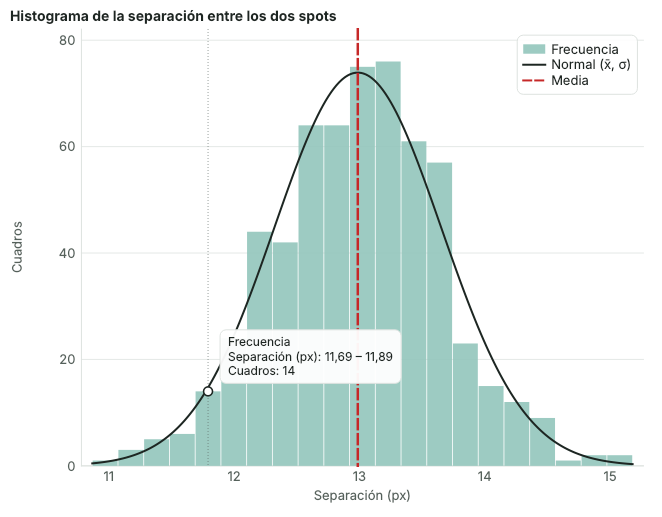
\includegraphics[width=\linewidth]{img/grafica_cursor.png}}
\end{minipage}

\subsection{Cuando no se detecta la estrella}

Si en el tramo hay menos de 10 cuadros con los dos puntos (la región quedó lejos, el video es de otra cosa o la estrella
está tan desenfocada que los puntos se tocan), las gráficas quedan vacías con un mensaje y los indicadores muestran
«—». No se dibuja nada que no sea una medición.

\captura[0.9\linewidth]{resultados_sin_datos.png}{Resultados de un video sin estrella: las gráficas dicen por qué están
vacías.}

% ------------------------------------------------------------------------------------------------ guardar y exportar
\section{Guardar y exportar}\label{sec:exportar}

\textbf{Guardar en el historial.} Escribe una etiqueta si quieres («Altair, noche 1», «tramo sin viento») y pulsa
\botonp{Guardar en historial}. Puedes guardar el mismo análisis varias veces, por ejemplo con otra etiqueta o después de
cambiar la escala; cada vez queda un registro nuevo y al lado del botón se lee su número («Guardado ✓ (\#12)»).

\textbf{Exportar} se hace en dos pasos, para que quede claro cuándo se crean los archivos:

\begin{capturam}{exportar}{La tarjeta \campo{Exportar} después de pulsar \botonp{Generar}.}[3]
\item Datos.
\item Gráficas.
\item Informe.
\item \boton{Cambiar carpeta…}
\item \botonp{Generar}.
\item \boton{Ver archivos}.
\end{capturam}

\begin{enumerate}
\item Elige los formatos (marcas \marcanum{1} a \marcanum{3}) y revisa la \textbf{carpeta de destino}. Por defecto es la de
los cuadros guardados o, si no guardaste cuadros, la del video. \boton{Cambiar carpeta…} elige otra \marcanum{4}.
\item \botonp{Generar} \marcanum{5} crea los archivos en ese momento, nunca antes. El mensaje de al lado dice cuántos se
crearon y con qué prefijo; \boton{Ver archivos} \marcanum{6} abre la carpeta en el explorador del sistema.
\end{enumerate}

\begin{table}[H]
\centering\small
\begin{tabularx}{\linewidth}{@{}l l Y@{}}
\toprule
Grupo & Formato & Contenido\\
\midrule
Datos & CSV & Dos archivos: las mediciones, una fila por cuadro (tiempo, posiciones, flujos, separación, componentes y si se usó), y el resumen.\\
 & Excel (.xlsx) & Dos hojas: el resumen y las mediciones.\\
 & JSON & El resumen y las mediciones, para programar.\\
 & NumPy (.npz) & Los arreglos por cuadro, para Python.\\
 & Tabla FITS & Las mediciones como tabla binaria, para software astronómico.\\
Gráficas & PDF solo gráficas & Todas las gráficas, una por página, sin texto.\\
 & PNG / SVG & Cada gráfica en un archivo.\\
Informe & PDF completo & El resumen con los parámetros, una nota del método y la calidad del cielo, y las gráficas.\\
\bottomrule
\end{tabularx}
\caption{Formatos de exportación.}
\end{table}

El nombre de los archivos es automático (el nombre del video más el tipo) y nunca se sobrescribe uno que ya exista: el
segundo lleva \ruta{\_2}, el tercero \ruta{\_3}, y así. Cada archivo lleva una línea con la cita de TurbuLENS.

\begin{nota}[Análisis sin guardar.]
Si abres otro video, vuelves a procesar o cierras TurbuLENS con un análisis de al menos 10 cuadros que no está en el
historial, aparece la pregunta «¿Guardarlo?» con \boton{Guardar}, \boton{Descartar} y \boton{Cancelar}. \boton{Guardar}
usa la etiqueta que hayas escrito en \menu{Resultados}.
\end{nota}

% ------------------------------------------------------------------------------------------------ historial
\section{Historial}\label{sec:historial}

El historial guarda cada análisis en una base de datos local, para comparar noches, estrellas y épocas del año. Es el
mismo en el modo medición y en el educativo; una columna dice en cuál se hizo cada análisis.

\captura{historial.png}{El \menu{Historial}. A la derecha, el seeing de cada análisis seleccionado.}

\begin{itemize}
\item La tabla muestra la fecha, el modo, la etiqueta, el video, el tramo, los cuadros, $\sigma$, el seeing, la escala y
las notas.
\item Marca las casillas de los análisis que quieras comparar: la gráfica de la derecha muestra su seeing.
\item \boton{Abrir en Resultados} vuelve a mostrar un análisis con todas sus gráficas, como el día que lo procesaste.
\item \boton{Etiqueta y notas…} cambia la etiqueta o agrega notas (el clima, quién grabó, qué estrella).
\item \boton{Eliminar seleccionados} los borra, después de preguntar.
\item \campo{Exportar los análisis seleccionados} funciona como en \menu{Resultados}: una tabla con una fila por
análisis, gráficas e informe.
\end{itemize}

\begin{consejo}[Una noche completa.]
Para seguir el seeing durante una noche, graba un video corto cada 15 o 30 minutos con la misma estrella y el mismo
montaje, procésalos con el mismo perfil y guarda cada uno con la hora en la etiqueta. En el historial, selecciónalos todos:
la gráfica muestra cómo cambió la turbulencia. Si además lees esa noche en el modo Satélite (capítulo~\ref{cap:satelite}),
puedes comparar las dos series.
\end{consejo}
